\section{Full Midpoint and RK4 refinement tables}
\label{app:solvers}

We use the same $R$ (repetitions) as in the main text: $\Delta t{=}1/R$ so that
$T{=}n$ is conserved ($n{=}9$ for ConvNeXt stage~3).
Tables~\ref{tab:app-cnx}--\ref{tab:app-r101} report the piecewise-constant schedule for Euler (RK1),
Midpoint (RK2) and RK4 on each pretrained model.
\Cref{tab:app-shared-t9} gives the same solvers for the weight-tied ConvNeXt-T at
fixed horizon $T{=}9$ ($9R$ applications of the shared block).
In every case the three integrators converge to the same continuous limit once the
step is fine enough; at $R{=}1$, RK4 already sits on that limit on every model, and
Midpoint does on ConvNeXt but not on the ResNets.
The ConvNeXt-T column is the evaluation of the final checkpoint; repeated evaluations
of the same checkpoint differ by up to two images ($0.004$ points) because of
nondeterministic GPU kernels.

\begin{table}[t]
    \centering
    \caption{ConvNeXt-T, piecewise-constant schedule, top-1 (\%).}
    \label{tab:app-cnx}
    \setlength{\tabcolsep}{4pt}
    \begin{tabular}{lrrr}
        \toprule
        $R$ & Euler & Mid & RK4 \\
        \midrule
        1   & 80.96 & 80.23 & 80.23 \\
        2   & 80.78 & 80.23 & 80.23 \\
        4   & 80.52 & 80.23 & 80.23 \\
        10  & 80.36 & 80.23 & 80.23 \\
        32  & 80.29 & 80.23 & 80.23 \\
        128 & 80.24 & 80.23 & 80.23 \\
        \bottomrule
    \end{tabular}
\end{table}

\begin{table}[t]
    \centering
    \caption{Swin-T, piecewise-constant schedule, top-1 (\%).}
    \label{tab:app-swin}
    \setlength{\tabcolsep}{4pt}
    \begin{tabular}{lrrr}
        \toprule
        $R$ & Euler & Mid & RK4 \\
        \midrule
        1   & 81.08 & 80.29 & 80.33 \\
        2   & 80.90 & 80.34 & 80.31 \\
        4   & 80.65 & 80.33 & 80.32 \\
        10  & 80.47 & 80.32 & 80.31 \\
        32  & 80.38 & 80.32 & 80.32 \\
        128 & 80.34 & 80.31 & 80.32 \\
        \bottomrule
    \end{tabular}
\end{table}

\begin{table}[t]
    \centering
    \caption{ResNet-50, piecewise-constant schedule, top-1 (\%).}
    \label{tab:app-r50}
    \setlength{\tabcolsep}{4pt}
    \begin{tabular}{lrrr}
        \toprule
        $R$ & Euler & Mid & RK4 \\
        \midrule
        1   & 80.34 & 78.94 & 79.42 \\
        2   & 80.06 & 79.41 & 79.43 \\
        4   & 79.84 & 79.44 & 79.43 \\
        10  & 79.61 & 79.44 & 79.43 \\
        32  & 79.50 & 79.43 & 79.44 \\
        128 & 79.45 & 79.43 & 79.43 \\
        \bottomrule
    \end{tabular}
\end{table}

\begin{table}[t]
    \centering
    \caption{ResNet-101, piecewise-constant schedule, top-1 (\%).}
    \label{tab:app-r101}
    \setlength{\tabcolsep}{4pt}
    \begin{tabular}{lrrr}
        \toprule
        $R$ & Euler & Mid & RK4 \\
        \midrule
        1   & 81.67 & 80.95 & 81.06 \\
        2   & 81.58 & 81.07 & 81.04 \\
        4   & 81.38 & 81.06 & 81.05 \\
        10  & 81.22 & 81.05 & 81.05 \\
        32  & 81.12 & 81.05 & 81.04 \\
        128 & 81.06 & 81.04 & 81.05 \\
        \bottomrule
    \end{tabular}
\end{table}

\begin{table}[t]
    \centering
    \caption{Shared ConvNeXt-T, fixed $T{=}9$ ($\Delta t{=}1/R$; $9R$ shared steps), top-1 (\%).}
    \label{tab:app-shared-t9}
    \setlength{\tabcolsep}{3.5pt}
    \small
    \begin{tabular}{lrrrrr}
        \toprule
        $R$ & Steps & $\Delta t$ & Euler & Mid & RK4 \\
        \midrule
        $1/9$   & 1     & 9      & 47.06 & 0.61  & 2.70 \\
        $2/9$   & 2     & 4.5    & 5.85  & 10.42 & 47.98 \\
        $3/9$   & 3     & 3      & 37.45 & 54.47 & 71.37 \\
        $4/9$   & 4     & 2.25   & 67.83 & 73.57 & 78.90 \\
        $5/9$   & 5     & 1.8    & 77.23 & 78.70 & 79.97 \\
        $6/9$   & 6     & 1.5    & 79.48 & 79.85 & 80.10 \\
        $7/9$   & 7     & 1.29   & 80.19 & 80.12 & 80.11 \\
        $8/9$   & 8     & 1.13   & 80.38 & 80.21 & 80.11 \\
        $1$     & 9     & 1      & 80.34 & 80.19 & 80.11 \\
        $4/3$   & 12    & 0.75   & 80.35 & 80.14 & 80.12 \\
        $2$     & 18    & 0.5    & 80.27 & 80.12 & 80.12 \\
        $32/9$  & 32    & 0.28   & 80.22 & 80.11 & 80.12 \\
        $128/9$ & 128   & 0.07   & 80.14 & 80.12 & 80.12 \\
        $1024/9$& 1024  & 0.009  & 80.12 & 80.12 & 80.12 \\
        $10000/9$&10000 & 0.0009 & 80.12 & --    & -- \\
        \bottomrule
    \end{tabular}
\end{table}

\paragraph{Large steps and the trained horizon.}
\Cref{fig:shared-fractional} plots the fractional rows of \cref{tab:app-shared-t9}.
Euler is not monotone in the number of steps: one step of $\Delta t{=}9$ keeps
$47.1\%$, two steps of $4.5$ fall to $5.9\%$ and three steps of $3$ recover $37.5\%$.
The two-step path overshoots.
On $500$ images, the stage-3 exit norm without the massive channel is $1370$ after two
steps, three times the native $458$, against $452$ after one step and $683$ after
three; the single step lands at a normal norm in a different direction (cosine $0.41$
to the native exit), which the decoder still partly classifies.
Varying the number of unit steps at $\Delta t{=}1$, or $\Delta t$ at nine steps,
peaks at $T{=}9$ in both cases (\cref{fig:horizon}).
Script for the overshoot measurements: \texttt{scripts/undo\_geometry\_audit.py}.

\begin{figure}[t]
    \centering
    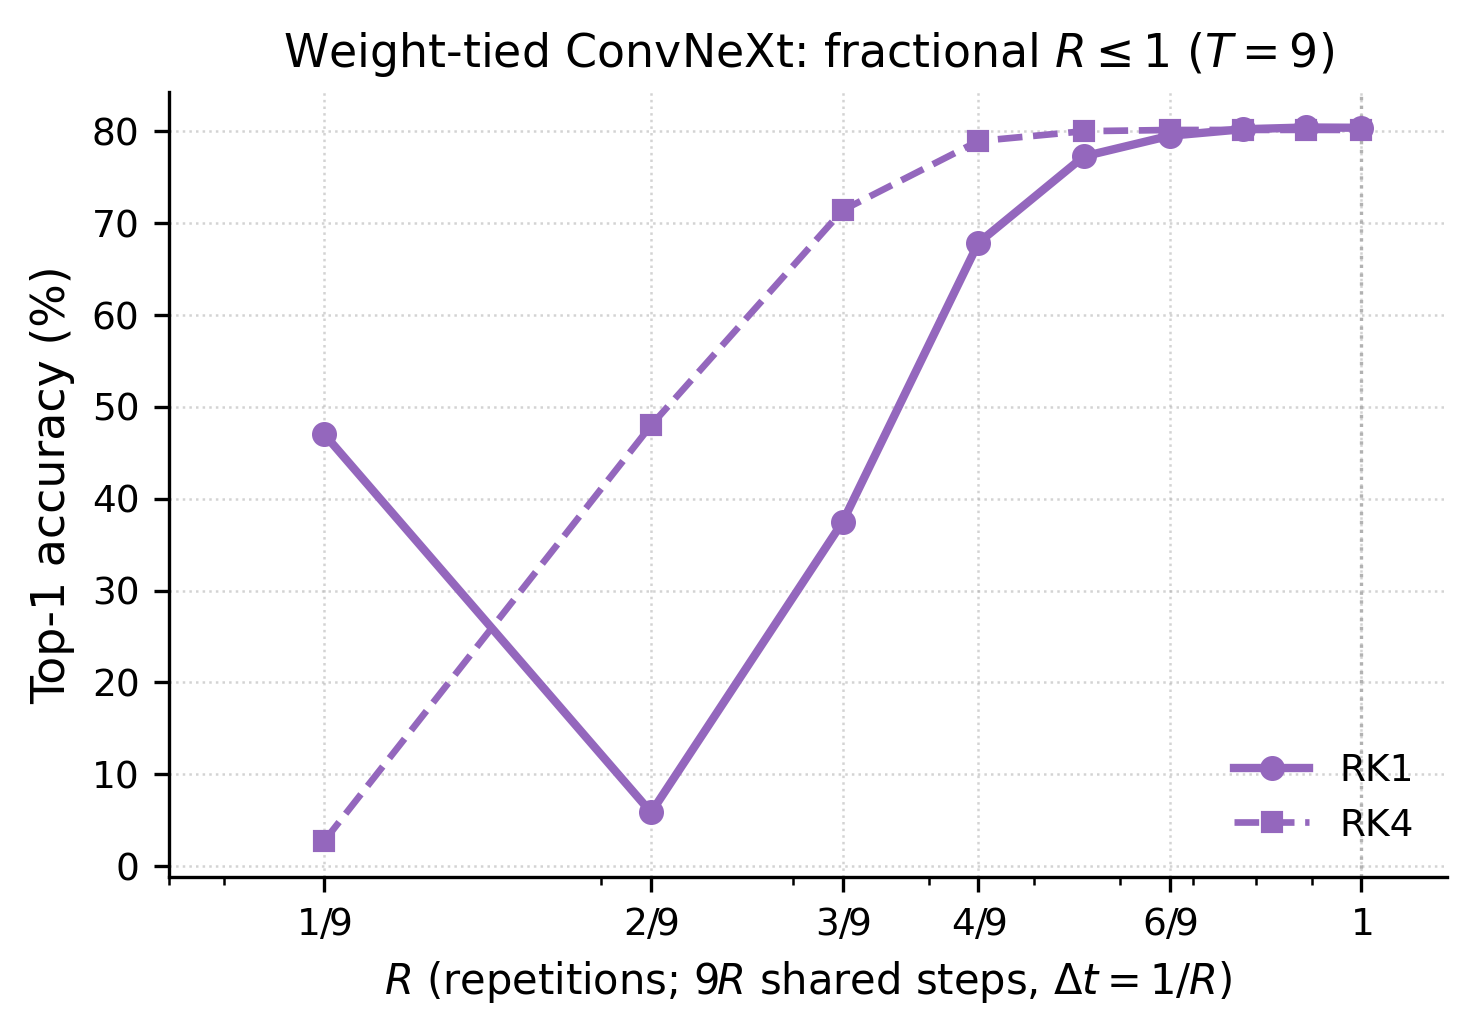
\includegraphics[width=\linewidth]{figures/shared_fractional.png}
    \caption{Weight-tied ConvNeXt-T at fixed $T{=}9$ with $9R\le 9$ steps
    (Euler solid, RK4 dashed).}
    \label{fig:shared-fractional}
\end{figure}

\begin{figure}[t]
    \centering
    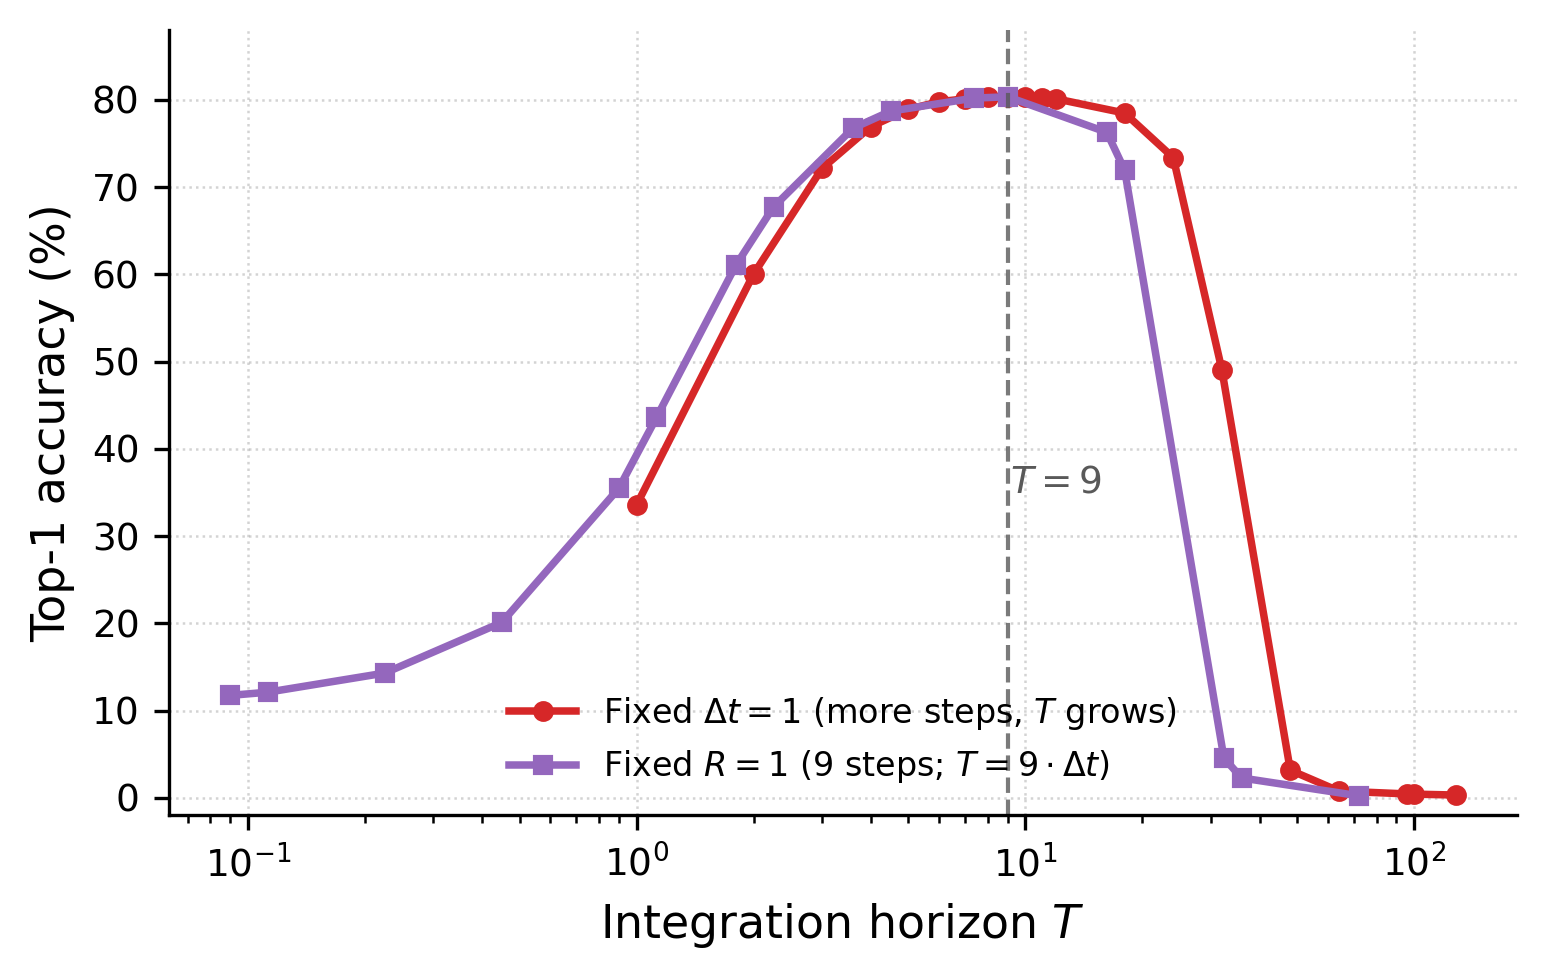
\includegraphics[width=\linewidth]{figures/horizon_ablation.png}
    \caption{Weight-tied ConvNeXt-T: top-1 against horizon $T$.
    Red: fixed $\Delta t{=}1$ and more steps.
    Purple: nine steps with varying $\Delta t$ ($T{=}9\,\Delta t$).
    Both peak at the trained horizon $T{=}9$.}
    \label{fig:horizon}
\end{figure}

